\documentclass[aspectratio=169,11pt]{beamer}

\usepackage[T1]{fontenc}
\usepackage{lmodern}
\usepackage{amsmath,amssymb}
\usepackage{booktabs}
\usepackage{tikz}
\usetikzlibrary{arrows.meta,positioning,calc,shapes.geometric,decorations.pathreplacing,backgrounds}
\usepackage{pgfplots}
\pgfplotsset{compat=1.17}

% ------------------------------------------------------------------
% Minimal theme
% ------------------------------------------------------------------
\definecolor{ink}{HTML}{222222}
\definecolor{muted}{HTML}{8A8A8A}
\definecolor{accent}{HTML}{2E86C1}
\definecolor{warm}{HTML}{CA6F1E}
\definecolor{good}{HTML}{1E8449}
\definecolor{bad}{HTML}{C0392B}
\definecolor{soft}{HTML}{F3F6F9}

\setbeamercolor{background canvas}{bg=white}
\setbeamercolor{normal text}{fg=ink}
\setbeamercolor{structure}{fg=accent}
\setbeamercolor{alerted text}{fg=warm}
\setbeamercolor{frametitle}{fg=ink,bg=white}
\setbeamerfont{frametitle}{size=\Large,series=\bfseries}
\setbeamertemplate{navigation symbols}{}
\setbeamertemplate{itemize item}{\color{accent}\raisebox{0.15ex}{\small$\bullet$}}
\setbeamertemplate{itemize subitem}{\color{muted}\raisebox{0.15ex}{\scriptsize$\bullet$}}
\setbeamertemplate{enumerate item}{\color{accent}\bfseries\insertenumlabel.}
\setbeamertemplate{frametitle}{%
  \vspace*{5mm}\insertframetitle\par\vspace{1.5mm}%
  {\color{accent}\rule{1.6cm}{1.6pt}}\vspace{-1mm}}
\setbeamertemplate{footline}{%
  \hfill{\scriptsize\color{muted}\insertframenumber}\hspace*{5mm}\vspace*{3mm}}

\AtBeginSection{%
  \begin{frame}[plain,noframenumbering]
    \vfill
    {\color{accent}\small\bfseries PART \thesection}\\[3pt]
    {\Huge\bfseries \insertsectionhead}
    \vfill
  \end{frame}}

% Reveal TikZ elements on given overlays: \node[visible on=<2->] ...
\tikzset{
  invisible/.style={opacity=0,text opacity=0},
  visible on/.style={alt={#1{}{invisible}}},
  alt/.code args={<#1>#2#3}{\alt<#1>{\pgfkeysalso{#2}}{\pgfkeysalso{#3}}},
  arr/.style={-{Stealth[length=2.2mm]}},
  tok/.style={draw=muted!60,rounded corners=2pt,minimum height=6.5mm,minimum width=11mm,font=\small},
  ctx/.style={tok,fill=accent!20,draw=accent!70},
  cen/.style={tok,fill=warm!35,draw=warm,font=\small\bfseries},
  dot/.style={circle,inner sep=1.6pt},
}

\newcommand{\vin}{\mathbf{v}}
\newcommand{\vout}{\mathbf{u}}
\newcommand{\muted}[1]{{\color{muted}#1}}
\newcommand{\key}[1]{{\color{accent}\textbf{#1}}}

% Sentence with a highlighted window (centre index #1, window 2)
\newcommand{\windowrow}[1]{%
  \foreach \w [count=\i from 0] in {the,quick,brown,fox,jumps,over,the,lazy,dog} {
    \pgfmathtruncatemacro{\d}{abs(\i-#1)}
    \ifnum\d=0 \tikzset{ws/.style={cen}}\else\ifnum\d<3 \tikzset{ws/.style={ctx}}\else\tikzset{ws/.style={tok}}\fi\fi
    \node[ws] (w\i) at (\i*1.5,0) {\w};
  }}

\title{word2vec}
\subtitle{How a computer learns what words mean, from text alone}
\date{}

\begin{document}

% ==================================================================
\begin{frame}[plain,noframenumbering]
  \vfill
  {\Huge\bfseries word2vec}\\[6pt]
  {\Large\color{muted} How a computer learns what words mean,\\ from nothing but text}\\[14pt]
  {\color{accent}\rule{2.4cm}{2pt}}\\[10pt]
  {\small\color{muted} Based on Mikolov et al., 2013}
  \vfill
\end{frame}

% ==================================================================
\begin{frame}{Today's plan}
  \begin{enumerate}
    \setlength{\itemsep}{10pt}
    \item<1-> \textbf{The problem}: why computers struggle with word meaning
    \item<1-> \textbf{The core idea}: learn meaning by predicting neighbours
    \item<1-> \textbf{How it learns}: negative sampling and hierarchical softmax
    \item<1-> \textbf{What you get}: similarity, analogies, and the limits
  \end{enumerate}
\end{frame}

% ==================================================================
\section{The problem}
% ==================================================================

\begin{frame}{To a computer, a word is just a symbol}
  Machine learning models work with \key{numbers}. So how do we turn words into numbers?

  \vspace{4mm}
  \onslide<2->{The simplest idea: \textbf{one-hot vectors}. One slot per word in the vocabulary.}

  \vspace{3mm}
  \centering
  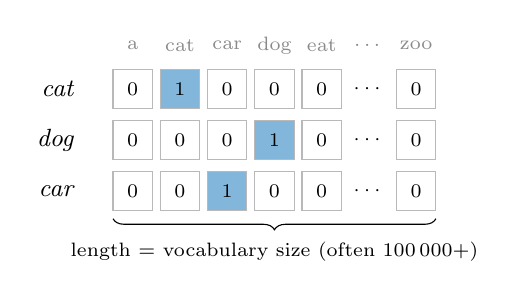
\begin{tikzpicture}[cell/.style={draw=muted!60,minimum size=5mm,inner sep=0pt,font=\scriptsize}]
    \begin{scope}[visible on=<2->]
      \foreach \lbl [count=\i from 0] in {a,cat,car,dog,eat,\dots,zoo}
        \node[font=\scriptsize,muted,rotate=0] at (\i*0.6+1.2,0.55) {\lbl};
      \foreach \w/\hot [count=\r from 0] in {cat/1,dog/3,car/2} {
        \node[anchor=east,font=\small] at (0.6,-\r*0.65) {\textit{\w}};
        \foreach \i in {0,...,6} {
          \ifnum\i=\hot
            \node[cell,fill=accent!60] at (\i*0.6+1.2,-\r*0.65) {1};
          \else\ifnum\i=5
            \node[cell,draw=none] at (\i*0.6+1.2,-\r*0.65) {$\cdots$};
          \else
            \node[cell] at (\i*0.6+1.2,-\r*0.65) {0};
          \fi\fi
        }
      }
      \draw[decorate,decoration={brace,amplitude=4pt,mirror}] (0.95,-1.65) -- (5.05,-1.65)
        node[midway,below=5pt,font=\scriptsize] {length = vocabulary size (often 100\,000+)};
    \end{scope}
  \end{tikzpicture}

  \vspace{3mm}
  \onslide<3->{\alert{Problem:} these numbers say nothing about what the words \emph{mean}.}
\end{frame}

% ------------------------------------------------------------------
\begin{frame}{One-hot: every word is equally far from every other}
  \begin{columns}[c]
    \begin{column}{0.45\textwidth}
      \centering
      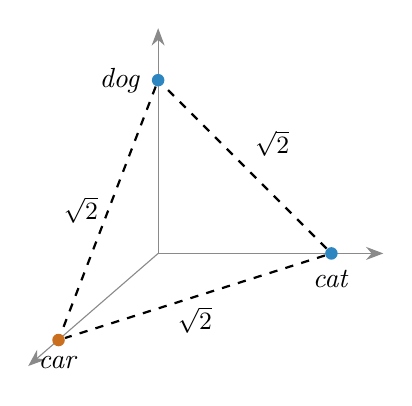
\begin{tikzpicture}[scale=1.1]
        \draw[arr,muted] (0,0) -- (2.6,0);
        \draw[arr,muted] (0,0) -- (0,2.6);
        \draw[arr,muted] (0,0) -- (-1.5,-1.3);
        \node[dot,fill=accent,label={below:\textit{cat}}] (cat) at (2,0) {};
        \node[dot,fill=accent,label={left:\textit{dog}}]  (dog) at (0,2) {};
        \node[dot,fill=warm,label={below:\textit{car}}]   (car) at (-1.15,-1) {};
        \begin{scope}[visible on=<2->]
          \draw[dashed,thick] (cat) -- (dog) node[midway,above right,font=\small] {$\sqrt2$};
          \draw[dashed,thick] (cat) -- (car) node[midway,below,font=\small] {$\sqrt2$};
          \draw[dashed,thick] (dog) -- (car) node[midway,left,font=\small] {$\sqrt2$};
        \end{scope}
      \end{tikzpicture}
    \end{column}
    \begin{column}{0.52\textwidth}
      \begin{itemize}
        \setlength{\itemsep}{8pt}
        \item<2-> \textit{cat} is exactly as far from \textit{dog} as from \textit{car}.
        \item<3-> Anything a model learns about \textit{cats} tells it \textbf{nothing} about \textit{dogs}.
        \item<4-> And the vectors are huge and almost all zeros.
      \end{itemize}
    \end{column}
  \end{columns}
\end{frame}

% ------------------------------------------------------------------
\begin{frame}{What we want instead: a map of meaning}
  \centering
  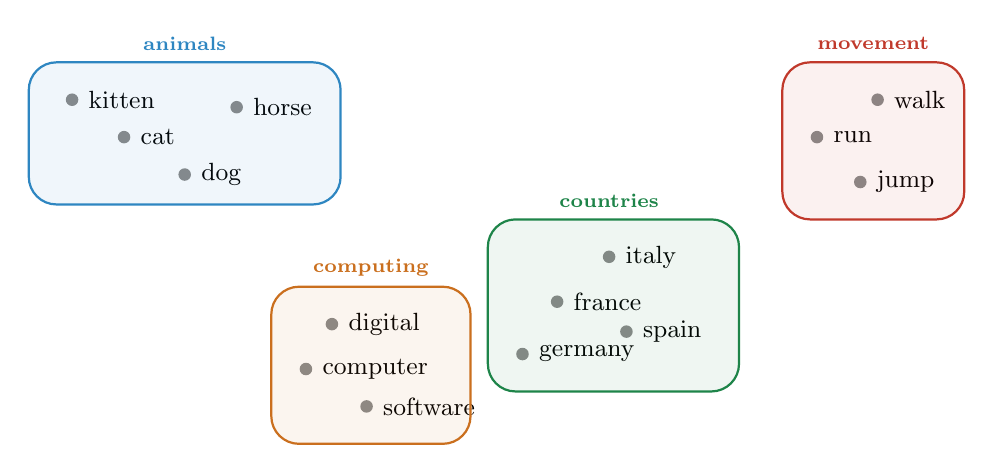
\begin{tikzpicture}[x=1.1cm,y=0.95cm,lbl/.style={font=\small}]
    % points
    \foreach \w/\x/\y in {cat/1/3.2,kitten/0.4/3.7,dog/1.7/2.7,horse/2.3/3.6,
                          france/6/1,spain/6.8/0.6,italy/6.6/1.6,germany/5.6/0.3,
                          computer/3.1/0.1,software/3.8/-0.4,digital/3.4/0.7,
                          run/9/3.2,walk/9.7/3.7,jump/9.5/2.6}
      \node[dot,fill=muted,label={[lbl]right:\w}] at (\x,\y) {};
    \begin{scope}[visible on=<2->]
      \draw[accent,thick,rounded corners=10pt,fill=accent,fill opacity=0.07] (-0.1,2.3) rectangle (3.5,4.2);
      \node[accent,font=\scriptsize\bfseries] at (1.7,4.45) {animals};
    \end{scope}
    \begin{scope}[visible on=<3->]
      \draw[good,thick,rounded corners=10pt,fill=good,fill opacity=0.07] (5.2,-0.2) rectangle (8.1,2.1);
      \node[good,font=\scriptsize\bfseries] at (6.6,2.35) {countries};
      \draw[warm,thick,rounded corners=10pt,fill=warm,fill opacity=0.07] (2.7,-0.9) rectangle (5.0,1.2);
      \node[warm,font=\scriptsize\bfseries] at (3.85,1.45) {computing};
      \draw[bad,thick,rounded corners=10pt,fill=bad,fill opacity=0.07] (8.6,2.1) rectangle (10.7,4.2);
      \node[bad,font=\scriptsize\bfseries] at (9.65,4.45) {movement};
    \end{scope}
  \end{tikzpicture}

  \vspace{2mm}
  \onslide<4->{Each word becomes a \key{short list of numbers} (say 200): a point in space.\\
  \textbf{Nearby points = similar meanings.} \muted{(We can only draw 2 dimensions.)}}
\end{frame}

% ------------------------------------------------------------------
\begin{frame}{Quick refresher: vectors and similarity}
  \begin{columns}[c]
    \begin{column}{0.4\textwidth}
      \centering
      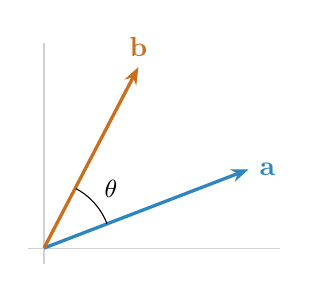
\begin{tikzpicture}[scale=1.0]
        \draw[muted!40] (-0.2,0) -- (3,0);
        \draw[muted!40] (0,-0.2) -- (0,2.6);
        \draw[arr,very thick,accent] (0,0) -- (2.6,1.0) node[right] {$\mathbf a$};
        \draw[arr,very thick,warm] (0,0) -- (1.2,2.3) node[above] {$\mathbf b$};
        \draw (0.8,0.31) arc[start angle=21,end angle=62,radius=0.85];
        \node[font=\small] at (0.85,0.75) {$\theta$};
      \end{tikzpicture}
    \end{column}
    \begin{column}{0.58\textwidth}
      \textbf{Dot product}: multiply matching entries, add them up
      \[ \mathbf a\cdot\mathbf b = a_1b_1 + a_2b_2 + \dots + a_db_d \]
      \onslide<2->{\textbf{Cosine similarity}: the dot product of the directions only
      \[ \cos\theta = \frac{\mathbf a\cdot\mathbf b}{\lVert\mathbf a\rVert\,\lVert\mathbf b\rVert} \]}
    \end{column}
  \end{columns}

  \vspace{0mm}
  \centering
  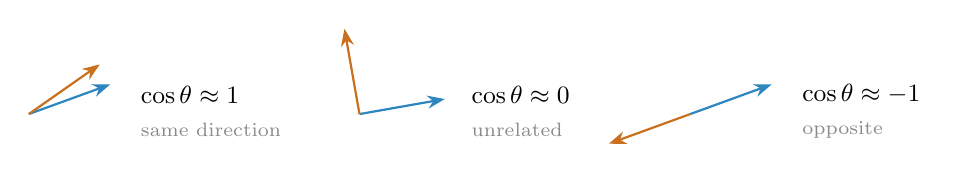
\begin{tikzpicture}[visible on=<3->]
    \foreach \x/\a/\b/\v/\t in {0/20/35/{\approx 1}/same direction,4.2/10/100/{\approx 0}/unrelated,8.4/20/200/{\approx -1}/opposite} {
      \begin{scope}[xshift=\x cm]
        \draw[arr,thick,accent] (0,0) -- (\a:1.1);
        \draw[arr,thick,warm] (0,0) -- (\b:1.1);
        \node[font=\small,anchor=west] at (1.3,0.25) {$\cos\theta\v$};
        \node[font=\scriptsize,muted,anchor=west] at (1.3,-0.2) {\t};
      \end{scope}
    }
  \end{tikzpicture}
\end{frame}

% ------------------------------------------------------------------
\begin{frame}{Where could meaning come from?}
  \begin{center}
    \Large\textit{``You shall know a word by the company it keeps.''}\\[2pt]
    \normalsize\muted{J.\,R.~Firth, linguist, 1957}
  \end{center}

  \vspace{3mm}
  \onslide<2->{Fill in the blank:
  \begin{center}
    \large I fed my \underline{\hspace{1.6cm}} and took it to the vet.
  \end{center}}
  \vspace{-2mm}
  \begin{center}
    \onslide<3->{{\color{good}cat \checkmark\quad dog \checkmark\quad rabbit \checkmark}\qquad
    {\color{bad}car $\times$\quad idea $\times$}}
  \end{center}

  \onslide<4->{\key{Distributional hypothesis}: words that appear in similar contexts have similar meanings.}\\[2pt]
  \onslide<5->{So if we capture each word's \emph{typical neighbours}, we capture its meaning.}
\end{frame}

% ==================================================================
\section{The core idea}
% ==================================================================

\begin{frame}{The trick: invent a prediction game}
  \begin{enumerate}
    \setlength{\itemsep}{7pt}
    \item<1-> Take a large amount of ordinary text (e.g.\ Wikipedia).
    \item<2-> Play a guessing game: \textbf{predict a word from its neighbours} (or the reverse).
    \item<3-> Give every word a vector, start them \textbf{random}, and adjust them to win the game.
    \item<4-> When training ends, \textbf{throw away the game and keep the vectors}.
  \end{enumerate}

  \vspace{5mm}
  \onslide<5->{%
  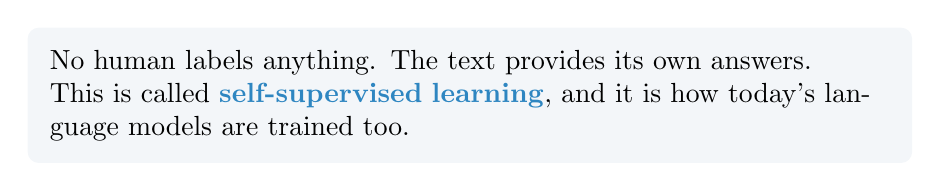
\begin{tikzpicture}
    \node[fill=soft,rounded corners=4pt,inner sep=8pt,text width=0.88\textwidth] {%
      No human labels anything. The text provides its own answers.\\
      This is called \key{self-supervised learning}, and it is how today's language models are trained too.};
  \end{tikzpicture}}
\end{frame}

% ------------------------------------------------------------------
\begin{frame}{Turning text into training examples}
  Slide a \key{window} over each sentence. The middle word is the \textcolor{warm}{\textbf{centre}};
  the words around it are its \textcolor{accent}{\textbf{context}}.

  \vspace{6mm}
  \centering
  \begin{tikzpicture}
    \only<1| handout:0>{\windowrow{2}}
    \only<2| handout:0>{\windowrow{3}}
    \only<3->{\windowrow{4}}
    \node[font=\scriptsize,muted] at (6,-0.75) {window = 2 words on each side};
  \end{tikzpicture}

  \vspace{6mm}
  \begin{tabular}{l}
    \only<1| handout:0>{Pairs: (brown, the) \;(brown, quick) \;(brown, fox) \;(brown, jumps)}%
    \only<2| handout:0>{Pairs: (fox, quick) \;(fox, brown) \;(fox, jumps) \;(fox, over)}%
    \only<3->{Pairs: (jumps, brown) \;(jumps, fox) \;(jumps, over) \;(jumps, the)}
  \end{tabular}

  \vspace{6mm}
  \onslide<4->{A billion words of text gives \textbf{billions} of free (centre, context) examples.}
\end{frame}

% ------------------------------------------------------------------
\begin{frame}{Two ways to play the game}
  \centering
  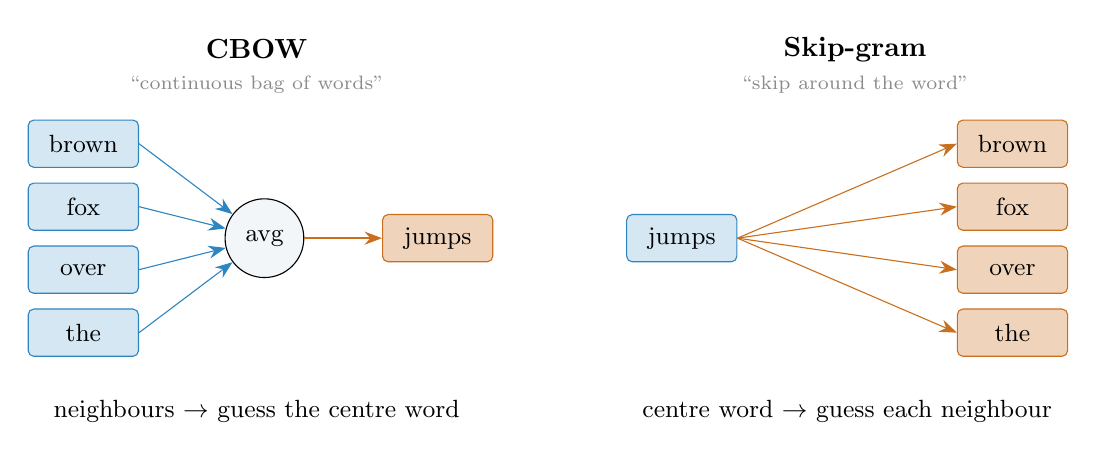
\begin{tikzpicture}[
      wn/.style={draw,rounded corners=2pt,minimum width=14mm,minimum height=6mm,font=\small},
      inw/.style={wn,fill=accent!20,draw=accent},
      outw/.style={wn,fill=warm!30,draw=warm}]
    \begin{scope}[visible on=<1->]
      \node[font=\bfseries] at (2.2,2.4) {CBOW};
      \node[font=\scriptsize,muted] at (2.2,1.95) {``continuous bag of words''};
      \node[inw] (c1) at (0,1.2)  {brown};
      \node[inw] (c2) at (0,0.4)  {fox};
      \node[inw] (c3) at (0,-0.4) {over};
      \node[inw] (c4) at (0,-1.2) {the};
      \node[draw,circle,fill=soft,minimum size=10mm,font=\small] (h) at (2.3,0) {avg};
      \node[outw] (o) at (4.5,0) {jumps};
      \foreach \i in {1,...,4} \draw[arr,accent] (c\i.east) -- (h);
      \draw[arr,warm,thick] (h) -- (o);
      \node[font=\small,text width=5.4cm,align=center] at (2.2,-2.2) {neighbours \(\to\) guess the centre word};
    \end{scope}
    \begin{scope}[xshift=7.6cm,visible on=<2->]
      \node[font=\bfseries] at (2.2,2.4) {Skip-gram};
      \node[font=\scriptsize,muted] at (2.2,1.95) {``skip around the word''};
      \node[inw] (s) at (0,0) {jumps};
      \node[outw] (t1) at (4.2,1.2)  {brown};
      \node[outw] (t2) at (4.2,0.4)  {fox};
      \node[outw] (t3) at (4.2,-0.4) {over};
      \node[outw] (t4) at (4.2,-1.2) {the};
      \foreach \i in {1,...,4} \draw[arr,warm] (s.east) -- (t\i.west);
      \node[font=\small,text width=5.4cm,align=center] at (2.1,-2.2) {centre word \(\to\) guess each neighbour};
    \end{scope}
  \end{tikzpicture}

  \vspace{0mm}
  \onslide<3->{CBOW is \textbf{faster}; skip-gram is slower but \textbf{better for rare words}. Both produce good vectors.}
\end{frame}

% ------------------------------------------------------------------
\begin{frame}{The whole model: two vectors per word and a dot product}
  \begin{columns}[c]
    \begin{column}{0.54\textwidth}
      Every word $w$ gets two vectors:
      \begin{itemize}
        \item $\vin_w$: the word as the \textcolor{accent}{\textbf{input}} \muted{(kept)}
        \item $\vout_w$: the word as a \textcolor{warm}{\textbf{neighbour}}
      \end{itemize}
      \vspace{3mm}
      \onslide<2->{How likely is $o$ to be a neighbour of $c$?\\[2pt]
      \hspace*{8mm}$\text{score} = \vin_c\cdot\vout_o$}\\[6pt]
      \onslide<3->{Squash the score into a probability\\ with the \key{sigmoid}:\\[2pt]
      \hspace*{8mm}$P = \sigma(\text{score}) = \dfrac{1}{1+e^{-\text{score}}}$}
    \end{column}
    \begin{column}{0.42\textwidth}
      \onslide<3->{%
      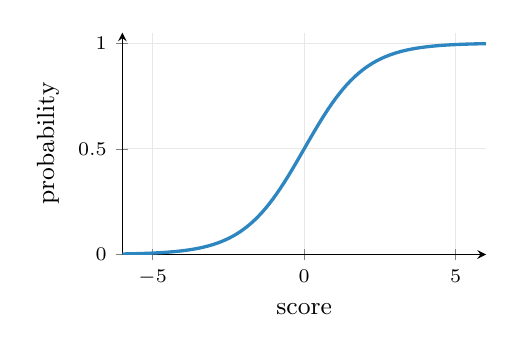
\begin{tikzpicture}
        \begin{axis}[width=6.2cm,height=4.4cm,xmin=-6,xmax=6,ymin=0,ymax=1.05,
          xlabel={score},ylabel={probability},xtick={-5,0,5},ytick={0,0.5,1},
          grid=major,grid style={muted!20},axis lines=left,
          label style={font=\small},tick label style={font=\scriptsize}]
          \addplot[accent,very thick,domain=-6:6,samples=100] {1/(1+exp(-x))};
        \end{axis}
      \end{tikzpicture}}
    \end{column}
  \end{columns}
  \vspace{1mm}
  \onslide<4->{\alert{That's all.} No deep network: just a dot product, a sigmoid, and lots of data.}
\end{frame}

% ==================================================================
\section{How it learns}
% ==================================================================

\begin{frame}{What does ``learning'' mean?}
  \begin{columns}[c]
    \begin{column}{0.5\textwidth}
      \begin{enumerate}
        \setlength{\itemsep}{5pt}
        \item<1-> Start with \textbf{random} vectors.
        \item<2-> Show the model one example; it makes a guess.
        \item<3-> Measure the \textbf{error}: how wrong was it?
        \item<4-> \textbf{Nudge} the numbers slightly to reduce the error.
        \item<5-> Repeat, millions of times.
      \end{enumerate}
      \vspace{3mm}
      \onslide<6->{\muted{The size of each nudge is the \textbf{learning rate}. It starts large and shrinks as training goes on.}}
    \end{column}
    \begin{column}{0.46\textwidth}
      \centering
      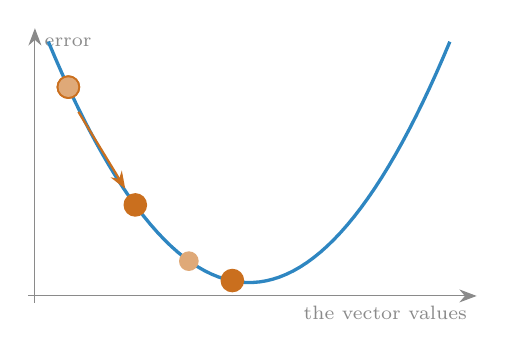
\begin{tikzpicture}[scale=0.85]
        \draw[arr,muted] (-3.3,0) -- (3.4,0) node[below left,font=\scriptsize] {the vector values};
        \draw[arr,muted] (-3.2,-0.1) -- (-3.2,4) node[below right,font=\scriptsize] {error};
        \draw[very thick,accent,domain=-3:3,samples=60] plot (\x,{0.4*\x*\x+0.2});
        \node[dot,fill=warm,minimum size=3mm,visible on=<1| handout:0>] at (-2.7,3.12) {};
        \node[dot,fill=warm,minimum size=3mm,visible on=<2-3| handout:0>] at (-2.7,3.12) {};
        \node[dot,fill=warm!60,minimum size=2.5mm,visible on=<4->] at (-2.7,3.12) {};
        \node[dot,fill=warm!60,minimum size=2.5mm,visible on=<5->] at (-1.7,1.36) {};
        \node[dot,fill=warm!60,minimum size=2.5mm,visible on=<5->] at (-0.9,0.52) {};
        \node[dot,fill=warm,minimum size=3mm,visible on=<4| handout:0>] at (-1.7,1.36) {};
        \node[dot,fill=warm,minimum size=3mm,visible on=<5->] at (-0.25,0.23) {};
        \draw[arr,warm,thick,visible on=<4->] (-2.55,2.75) -- (-1.85,1.6);
      \end{tikzpicture}
    \end{column}
  \end{columns}
\end{frame}

% ------------------------------------------------------------------
\begin{frame}{The obvious approach: a probability for every word}
  To guess the neighbour of \textit{fox}, score \textbf{every} word in the vocabulary and turn the
  scores into probabilities that add up to 1 (the \key{softmax}):
  \[ P(o\mid c) = \frac{e^{\,\vin_c\cdot\vout_o}}{\sum_{w\,\in\,\text{all words}} e^{\,\vin_c\cdot\vout_w}} \]

  \centering
  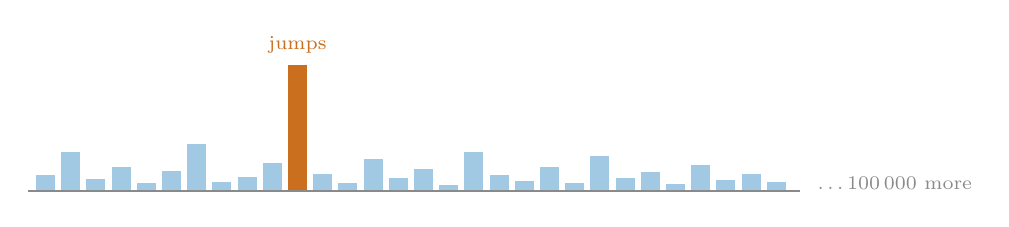
\begin{tikzpicture}[visible on=<2->]
    \foreach \h [count=\i from 0] in {0.2,0.5,0.15,0.3,0.1,0.25,0.6,0.12,0.18,0.35,1.6,0.22,0.1,0.4,0.16,0.28,0.08,0.5,0.2,0.13,0.3,0.1,0.45,0.17,0.24,0.09,0.33,0.14,0.21,0.11} {
      \ifnum\i=10
        \fill[warm] (\i*0.32,0) rectangle ++(0.24,\h);
      \else
        \fill[accent!45] (\i*0.32,0) rectangle ++(0.24,\h);
      \fi
    }
    \node[font=\scriptsize,warm] at (3.32,1.85) {jumps};
    \draw[muted] (-0.1,0) -- (9.7,0);
    \node[font=\scriptsize,muted,anchor=west] at (9.8,0.1) {\dots 100\,000 more};
  \end{tikzpicture}

  \vspace{3mm}
  \onslide<3->{\alert{Problem:} the bottom of the fraction needs \textbf{100\,000 dot products} for \emph{every}
  example, and there are billions of examples. Far too slow.}
\end{frame}

% ------------------------------------------------------------------
\begin{frame}{Fix \#1: negative sampling. Ask ``real or fake?''}
  Replace \emph{``which of 100\,000 words is the neighbour?''} with a yes/no question:
  \emph{``is this pair real?''}

  \vspace{2mm}
  \centering
  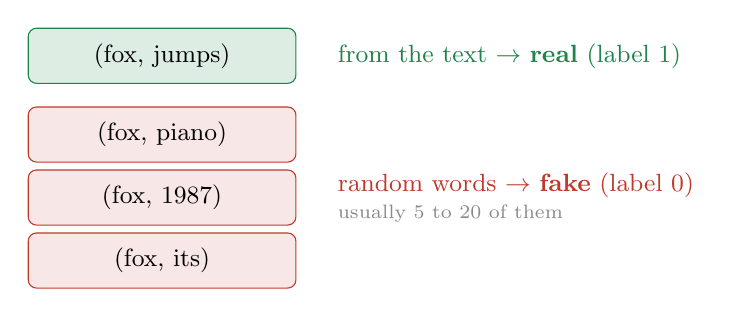
\begin{tikzpicture}[pair/.style={draw,rounded corners=3pt,minimum width=3.4cm,minimum height=7mm,font=\small}]
    \node[pair,fill=good!15,draw=good] (p) at (0,0) {(fox, jumps)};
    \node[right=4mm of p,good,font=\small] {from the text \(\to\) \textbf{real} (label 1)};
    \begin{scope}[visible on=<2->]
      \node[pair,fill=bad!12,draw=bad] (n1) at (0,-1.0) {(fox, piano)};
      \node[pair,fill=bad!12,draw=bad] (n2) at (0,-1.8) {(fox, 1987)};
      \node[pair,fill=bad!12,draw=bad] (n3) at (0,-2.6) {(fox, its)};
      \node[right=4mm of n2,bad,font=\small,align=left] {random words \(\to\) \textbf{fake} (label 0)\\[-1pt]\scriptsize\muted{usually 5 to 20 of them}};
    \end{scope}
  \end{tikzpicture}

  \vspace{2mm}
  \raggedright
  \onslide<3->{The model only has to tell real pairs from random ones: \key{6 dot products instead of 100\,000}.}\\[3pt]
  \onslide<4->{\muted{The random ``fake'' words are called \emph{negative samples}.}}
\end{frame}

% ------------------------------------------------------------------
\begin{frame}{The learning rule: error = label $-$ prediction}
  \centering
  \begin{tabular}{lcccl}
    \toprule
    pair & label & model says & error & what happens \\
    \midrule
    \uncover<2->{(fox, jumps) & 1 & 0.30 & \textcolor{good}{$+0.70$} & pull together, strongly} \\
    \uncover<3->{(fox, piano) & 0 & 0.60 & \textcolor{bad}{$-0.60$} & push apart} \\
    \uncover<4->{(fox, its)   & 0 & 0.05 & $-0.05$ & almost nothing} \\
    \bottomrule
  \end{tabular}

  \vspace{6mm}
  \raggedright
  \onslide<5->{Each vector moves a small step in the direction of the other, scaled by the error:
  \[ \vout_o \;\leftarrow\; \vout_o + \eta\cdot\text{error}\cdot\vin_c
     \qquad\qquad
     \vin_c \;\leftarrow\; \vin_c + \eta\cdot\text{error}\cdot\vout_o \]}
  \onslide<6->{\muted{$\eta$ is the learning rate.} Big mistakes \(\to\) big corrections; good guesses \(\to\) tiny ones.}
\end{frame}

% ------------------------------------------------------------------
\begin{frame}{Pull and push, in pictures}
  \centering
  \begin{tikzpicture}[scale=1.5]
    \draw[muted!30] (-2.4,0) -- (2.6,0);
    \draw[muted!30] (0,-0.1) -- (0,2.3);
    % before
    \only<1| handout:0>{
      \draw[arr,very thick,accent] (0,0) -- (70:2) node[above] {$\vin_{\text{fox}}$};
    }
    \only<2->{
      \draw[arr,thick,accent!35,dashed] (0,0) -- (70:2);
      \draw[arr,very thick,accent] (0,0) -- (42:2) node[above right] {$\vin_{\text{fox}}$};
      \draw[->,accent,thick] (68:1.4) arc[start angle=68,end angle=45,radius=1.4];
    }
    \only<1| handout:0>{
      \draw[arr,very thick,good] (0,0) -- (15:2) node[right] {$\vout_{\text{jumps}}$};
      \draw[arr,very thick,bad] (0,0) -- (125:2) node[above left] {$\vout_{\text{piano}}$};
    }
    \only<2->{
      \draw[arr,very thick,good] (0,0) -- (25:2) node[right] {$\vout_{\text{jumps}}$};
      \draw[arr,very thick,bad] (0,0) -- (140:2) node[above left] {$\vout_{\text{piano}}$};
      \draw[arr,thick,good!35,dashed] (0,0) -- (15:2);
      \draw[arr,thick,bad!35,dashed] (0,0) -- (125:2);
    }
  \end{tikzpicture}

  \vspace{4mm}
  \only<1| handout:0>{Before the update: \textit{fox} is not especially close to its real neighbour \textit{jumps}.}%
  \only<2->{After: \textit{fox} and \textit{jumps} \textcolor{good}{rotate towards each other};
  \textit{piano} is \textcolor{bad}{pushed away}.}
\end{frame}

% ------------------------------------------------------------------
\begin{frame}{Why similar words end up close together}
  \centering
  \begin{tikzpicture}[scale=1.0,
      ctxw/.style={dot,fill=warm},
      word/.style={dot,fill=accent,minimum size=2.4mm}]
    \foreach \w/\x/\y in {fed/4.0/3.0,vet/4.8/2.4,pet/3.4/2.1}
      \node[ctxw,label={[font=\small,warm]above:\w}] (\w) at (\x,\y) {};
    \foreach \w/\x/\y in {drive/9.8/2.9,engine/10.6/2.3}
      \node[ctxw,label={[font=\small,warm]above:\w}] (\w) at (\x,\y) {};
    \node[font=\scriptsize,muted] at (4,3.9) {context vectors $\vout$};

    \only<1-2| handout:0>{
      \node[word,label={[font=\small]below:cat}] (cat) at (0.3,0.2) {};
      \node[word,label={[font=\small]below:dog}] (dog) at (7.3,0.1) {};
      \node[word,label={[font=\small]below:car}] (car) at (5.5,-0.6) {};
    }
    \only<2| handout:0>{
      \foreach \t in {fed,vet,pet} {
        \draw[arr,accent!70,thick] (cat) -- ($(cat)!0.35!(\t)$);
        \draw[arr,accent!70,thick] (dog) -- ($(dog)!0.35!(\t)$);
      }
      \draw[arr,accent!70,thick] (car) -- ($(car)!0.3!(drive)$);
      \draw[arr,accent!70,thick] (car) -- ($(car)!0.3!(engine)$);
    }
    \only<3->{
      \node[word,label={[font=\small]left:cat}] at (3.7,1.0) {};
      \node[word,label={[font=\small]right:dog}] at (4.3,0.9) {};
      \node[word,label={[font=\small]below:car}] at (9.6,1.3) {};
      \draw[accent,thick,dashed,rounded corners=8pt] (2.8,0.5) rectangle (5.2,1.4);
    }
  \end{tikzpicture}

  \vspace{4mm}
  \only<1| handout:0>{\textit{cat} and \textit{dog} start far apart, at random positions.}%
  \only<2| handout:0>{Both keep appearing next to \textit{fed}, \textit{vet}, \textit{pet}, so both get pulled towards the same places.}%
  \only<3->{They end up \textbf{close together}. Nobody told the model that cats are like dogs: it follows from \key{shared contexts}.}
\end{frame}

% ------------------------------------------------------------------
\begin{frame}{Fix \#2: hierarchical softmax. Find the word by asking ``left or right?''}
  \begin{columns}[c]
    \begin{column}{0.5\textwidth}
      \begin{itemize}
        \setlength{\itemsep}{5pt}
        \item<1-> Put all words at the \textbf{leaves} of a binary tree.
        \item<2-> Each branching point has its own vector and asks a yes/no question: \emph{go left or right?}
        \item<3-> P(word) = product of the probabilities along its path.
        \item<5-> \key{100\,000 words \(\to\) about 17 questions} ($\log_2 100\,000$).
      \end{itemize}
    \end{column}
    \begin{column}{0.48\textwidth}
      \centering
      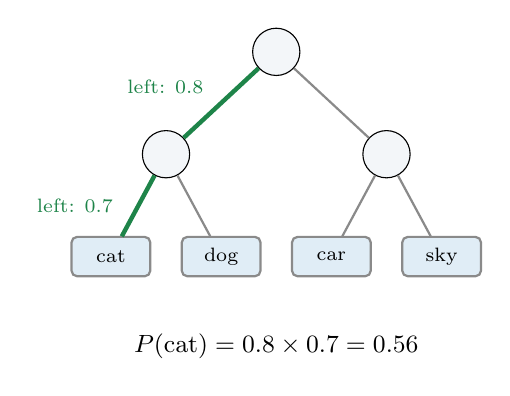
\begin{tikzpicture}[
          level distance=13mm,
          level 1/.style={sibling distance=28mm},
          level 2/.style={sibling distance=14mm},
          inner/.style={circle,draw,fill=soft,minimum size=6mm,font=\scriptsize},
          leaf/.style={rounded corners=2pt,draw,fill=accent!15,font=\scriptsize,minimum height=5mm,minimum width=10mm},
          edge from parent/.style={draw,thick,muted}]
        \node[inner] (r) {}
          child { node[inner] (a) {}
            child { node[leaf] (cat) {cat} }
            child { node[leaf] {dog} } }
          child { node[inner] {}
            child { node[leaf] {car} }
            child { node[leaf] {sky} } };
        \begin{scope}[visible on=<4->]
          \draw[ultra thick,good] (r) -- (a);
          \draw[ultra thick,good] (a) -- (cat);
          \node[good,font=\scriptsize,above left=0mm and 1mm] at ($(r)!0.5!(a)$) {left: 0.8};
          \node[good,font=\scriptsize,left=2mm] at ($(a)!0.5!(cat)$) {left: 0.7};
          \node[font=\small,below=6mm] at (cat.south -| r) {$P(\text{cat}) = 0.8 \times 0.7 = 0.56$};
        \end{scope}
      \end{tikzpicture}
    \end{column}
  \end{columns}
\end{frame}

% ------------------------------------------------------------------
\begin{frame}{A smarter tree: frequent words get short paths}
  \begin{columns}[c]
    \begin{column}{0.36\textwidth}
      \centering
      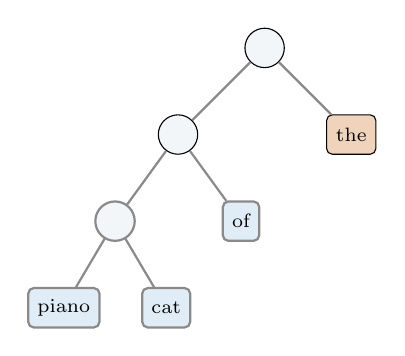
\begin{tikzpicture}[
          level distance=11mm,
          level 1/.style={sibling distance=22mm},
          level 2/.style={sibling distance=16mm},
          level 3/.style={sibling distance=13mm},
          inner/.style={circle,draw,fill=soft,minimum size=5mm},
          leaf/.style={rounded corners=2pt,draw,fill=accent!15,font=\scriptsize,minimum height=5mm},
          edge from parent/.style={draw,thick,muted}]
        \node[inner] {}
          child { node[inner] {}
            child { node[inner] {}
              child { node[leaf] {piano} }
              child { node[leaf] {cat} } }
            child { node[leaf] {of} } }
          child { node[leaf,fill=warm!30] {the} };
      \end{tikzpicture}

      \vspace{2mm}
      {\scriptsize A \key{Huffman tree}, as used in file compression}
    \end{column}
    \begin{column}{0.62\textwidth}
      \onslide<2->{%
      \small
      \begin{tabular}{@{}p{2.3cm}p{2.5cm}p{2.5cm}@{}}
        \toprule
        & \textbf{Negative sampling} & \textbf{Hierarchical softmax} \\
        \midrule
        Question & real or fake pair? & left or right? \\
        Work per example & 5--20 checks & $\sim$17 checks \\
        Tends to be better for & frequent words & rare words \\
        \bottomrule
      \end{tabular}}

      \vspace{4mm}
      \onslide<3->{Same idea in both: \key{replace one enormous choice with a few yes/no choices}.}
    \end{column}
  \end{columns}
\end{frame}

% ------------------------------------------------------------------
\begin{frame}{Two refinements that help a lot}
  \begin{columns}[t]
    \begin{column}{0.48\textwidth}
      \textbf{1. Skip some very common words}\\[2pt]
      \small \textit{the} makes up about 6\% of English text and says little about its neighbours.
      Randomly \key{drop most occurrences} of very frequent words:
      \begin{itemize}
        \item training gets much faster
        \item rare words get relatively more attention
      \end{itemize}
    \end{column}
    \begin{column}{0.48\textwidth}
      \onslide<2->{%
      \textbf{2. Pick fake words fairly}\\[2pt]
      \small Draw negative samples in proportion to \key{frequency$^{3/4}$}, not raw frequency.
      This gives rare words a better chance:\\[4pt]
      \begin{tabular}{lrr}
        \toprule
        word & share of text & share of fakes \\
        \midrule
        the   & 90\%   & 82\% \\
        of    & 9\%    & 15\% \\
        cat   & 0.9\%  & 2.6\% \\
        piano & 0.09\% & 0.46\% \\
        \bottomrule
      \end{tabular}\\[2pt]
      {\scriptsize\muted{Toy 4-word vocabulary.}}}
    \end{column}
  \end{columns}
\end{frame}

% ==================================================================
\section{What you get}
% ==================================================================

\begin{frame}{Nearest neighbours (real output)}
  \muted{\small Trained on \textit{text8} (17 million words of Wikipedia), 200-dimensional vectors.
  Numbers are cosine similarity.}

  \vspace{4mm}
  \centering
  \begin{tabular}{lr}
    \multicolumn{2}{c}{\key{france}} \\ \midrule
    spain & 0.64 \\ italy & 0.63 \\ french & 0.61 \\ germany & 0.58 \\ belgium & 0.57
  \end{tabular}
  \hspace{10mm}
  \uncover<2->{%
  \begin{tabular}{lr}
    \multicolumn{2}{c}{\key{cat}} \\ \midrule
    meow & 0.60 \\ cats & 0.59 \\ feline & 0.57 \\ dog & 0.56 \\ kitten & 0.55
  \end{tabular}}
  \hspace{10mm}
  \uncover<3->{%
  \begin{tabular}{lr}
    \multicolumn{2}{c}{\key{computer}} \\ \midrule
    computers & 0.69 \\ computing & 0.65 \\ software & 0.57 \\ digital & 0.53 \\ technology & 0.53
  \end{tabular}}

  \vspace{6mm}
  \raggedright
  \onslide<4->{The model was never told any of this. It learned it from which words appear near which.}
\end{frame}

% ------------------------------------------------------------------
\begin{frame}{Analogies with vector arithmetic}
  \begin{columns}[c]
    \begin{column}{0.45\textwidth}
      \centering
      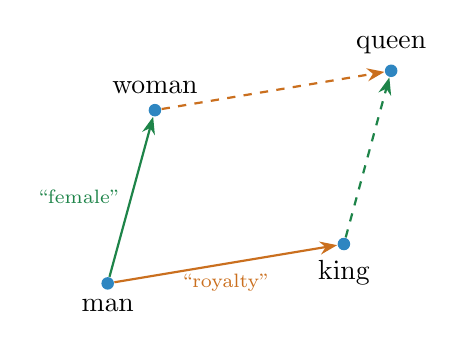
\begin{tikzpicture}[scale=1.0,w/.style={dot,fill=accent}]
        \node[w,label={below:man}]   (man)   at (0,0) {};
        \node[w,label={below:king}]  (king)  at (3,0.5) {};
        \node[w,label={above:woman}] (woman) at (0.6,2.2) {};
        \node[w,label={above:queen},visible on=<3->] (queen) at (3.6,2.7) {};
        \draw[arr,thick,warm,visible on=<1->] (man) -- (king) node[midway,below,font=\scriptsize] {``royalty''};
        \draw[arr,thick,good,visible on=<2->] (man) -- (woman) node[midway,left,font=\scriptsize] {``female''};
        \draw[arr,thick,good,dashed,visible on=<3->] (king) -- (queen);
        \draw[arr,thick,warm,dashed,visible on=<3->] (woman) -- (queen);
      \end{tikzpicture}
    \end{column}
    \begin{column}{0.53\textwidth}
      \onslide<3->{\[ \vin_{\text{king}} - \vin_{\text{man}} + \vin_{\text{woman}} \approx\; ? \]}
      \onslide<4->{\small Real answers (closest word to the result):\\[3pt]
      \begin{tabular}{@{}ll@{}}
        king $-$ man $+$ woman & \(\to\) \textbf{queen} \muted{(0.60)} \\
        paris $-$ france $+$ germany & \(\to\) \textbf{berlin} \muted{(0.65)} \\
      \end{tabular}}

      \vspace{3mm}
      \onslide<5->{\small It doesn't always work:\\[3pt]
      \begin{tabular}{@{}ll@{}}
        bigger $-$ big $+$ small & \(\to\) \textcolor{bad}{larger} \muted{(0.66)}\\
        & \muted{\phantom{\(\to\)} then} smaller \muted{(0.65)}
      \end{tabular}}
    \end{column}
  \end{columns}

  \vspace{4mm}
  \onslide<6->{Relationships such as gender, capital-of and verb tense become \key{consistent directions} in the space.}
\end{frame}

% ------------------------------------------------------------------
\begin{frame}{Limitations}
  \begin{itemize}
    \setlength{\itemsep}{7pt}
    \item<1-> \textbf{One vector per word.} \textit{bank} (of a river) and \textit{bank} (money) share one blended vector.
    \item<2-> \textbf{Context is ignored at use time.} A word gets the same vector in every sentence.
    \item<3-> \textbf{Unknown words get nothing.} A word never seen in training has no vector, and spelling isn't used.
    \item<4-> \textbf{It learns the biases in its text.} E.g.\ \textit{man : programmer :: woman : homemaker}
          was found in vectors trained on news (Bolukbasi et al., 2016).
    \item<5-> \textbf{It needs a lot of text} to produce good vectors.
  \end{itemize}
\end{frame}

% ------------------------------------------------------------------
\begin{frame}{What came next}
  \centering
  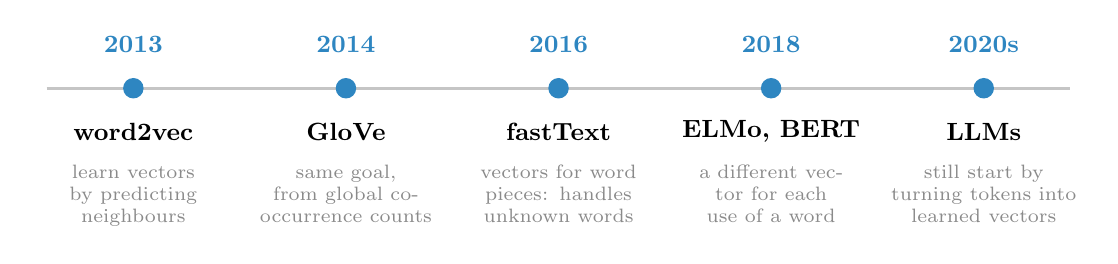
\begin{tikzpicture}[ev/.style={font=\small,text width=2.45cm,align=center}]
    \draw[very thick,muted!50] (0.2,0) -- (13.2,0);
    \foreach \x/\yr/\name/\desc/\s in {
        1.3/2013/word2vec/{learn vectors by predicting neighbours}/1,
        4.0/2014/GloVe/{same goal, from global co-occurrence counts}/2,
        6.7/2016/fastText/{vectors for word pieces: handles unknown words}/3,
        9.4/2018/{ELMo, BERT}/{a different vector for each use of a word}/4,
        12.1/2020s/LLMs/{still start by turning tokens into learned vectors}/5} {
      \begin{scope}[visible on=<\s->]
        \node[dot,fill=accent,minimum size=2.6mm] at (\x,0) {};
        \node[font=\small\bfseries,accent] at (\x,0.55) {\yr};
        \node[ev,font=\small\bfseries] at (\x,-0.55) {\name};
        \node[ev,font=\scriptsize,muted,anchor=north] at (\x,-0.85) {\desc};
      \end{scope}
    }
  \end{tikzpicture}

  \vspace{8mm}
  \raggedright
  \onslide<6->{The core idea of word2vec, \key{meaning from context, learned by prediction}, is still at the heart of modern language models.}
\end{frame}

% ------------------------------------------------------------------
\begin{frame}{Takeaways}
  \begin{enumerate}
    \setlength{\itemsep}{10pt}
    \item<1-> \textbf{Meaning comes from context}: words with similar neighbours are similar.
    \item<2-> \textbf{Invent a prediction game, keep the vectors}: the text provides its own labels.
    \item<3-> \textbf{Make it cheap}: negative sampling or hierarchical softmax turn one huge choice into a few yes/no choices.
    \item<4-> \textbf{Geometry encodes meaning}: distance means similarity, and directions capture relationships.
  \end{enumerate}
\end{frame}

% ------------------------------------------------------------------
\begin{frame}{Questions?}
  \vspace{4mm}
  \textbf{Further reading}\\[4pt]
  \small
  \begin{itemize}
    \setlength{\itemsep}{4pt}
    \item Mikolov, Chen, Corrado, Dean. \emph{Efficient Estimation of Word Representations in Vector Space}, 2013.
    \item Mikolov, Sutskever, Chen, Corrado, Dean. \emph{Distributed Representations of Words and Phrases and their Compositionality}, NeurIPS 2013.
    \item Goldberg, Levy. \emph{word2vec Explained}, arXiv:1402.3722, 2014.
    \item Jay Alammar. \emph{The Illustrated Word2vec} (blog post), 2019.
    \item Bolukbasi et al. \emph{Man is to Computer Programmer as Woman is to Homemaker?}, NeurIPS 2016.
  \end{itemize}
\end{frame}

\end{document}
